\documentclass[ignorenonframetext,xcolor=dvipsnames]{beamer}

\definecolor{mun}{RGB}{134,38,51}
\definecolor{mun2}{RGB}{99,102,106}
%\definecolor{mun}{cmyk}{0,.3922,.2392,.1686}
\definecolor{code}{RGB}{0, 0, 128}
\definecolor{code}{gray}{0.95}

\mode<presentation>
{
%  \usetheme{boxes}
%  \usetheme{default}
%  \usetheme{Montpellier}
%  \usetheme{Singapore}
%   \usetheme{Rochester}
%  \usecolortheme{crane}
%  \usecolortheme{dolphin}
%  \usecolortheme{lily}
%  \usecolortheme{orchid}
  \usecolortheme{rose}
  \setbeamercovered{transparent}
%  \usefonttheme[onlymath]{serif}
  \setbeamercolor*{structure}{bg=mun,fg=mun}
  \setbeamercolor*{palette primary}{use=structure,fg=white,bg=structure.fg}
  \setbeamercolor*{palette secondary}{use=structure,fg=white,bg=structure.fg}
  \setbeamercolor*{palette tertiary}{use=structure,fg=white,bg=black}
  \setbeamercolor*{palette quaternary}{fg=white,bg=black}
  \setbeamercolor{section in toc}{fg=black,bg=white}
  \setbeamercolor{alerted text}{use=structure,fg=structure.fg!50!black!80!black}
  \setbeamercolor{titlelike}{parent=palette primary,fg=structure.fg!50!black}
  \setbeamercolor{frametitle}{bg=mun,fg=white}
  \setbeamercolor*{titlelike}{parent=palette primary}

  \setbeamercolor{normal text}{fg=black!90}
  \setbeamercolor{math text}{fg=black}
  \setbeamercolor{quote}{bg=gray!20}
  \setbeamercolor{quotation}{bg=gray!20}
  \setbeamerfont{cite}{size=\scriptsize}
  \setbeamerfont{quote}{size=\footnotesize}
  \setbeamerfont{quotation}{size=\footnotesize}
  \setbeamercolor{red text}{fg=red!75!black}
  \setbeamertemplate{bibliography item}[triangle]
  \setbeamertemplate{enumerate item}[square]
  \setbeamertemplate{blocks}[rounded][shadow=true]
  \setbeamertemplate{navigation symbols}{}
  \setbeamertemplate{footline}[frame number]
}
\usepackage{tcolorbox}
\usepackage{amsmath}
\usepackage{physics}
\usepackage{pgf}
\usepackage[english]{babel}
\usepackage[latin1]{inputenc}
\usepackage{times}
\usepackage[T1]{fontenc}
\usepackage{multicol}
\usepackage{multirow}
\usepackage{fancyvrb}
\usepackage{tabularx}
\usepackage{amsmath}
\usepackage{bbm}
\usepackage{alltt}
\usepackage{hyperref}
\hypersetup{
    colorlinks=true,
    linkcolor=blue,
    filecolor=magenta,      
    urlcolor=blue,
}
\usepackage{minted}
\newminted{cypher}{autogobble,bgcolor=code,breakbytoken,frame=single,framesep=3pt}
\newminted{R}{autogobble,bgcolor=code,breakbytoken,frame=single,framesep=3pt}
\newminted{text}{autogobble,bgcolor=code,breakbytoken,frame=single,framesep=3pt}
\newminted{sql}{autogobble,bgcolor=code,breakbytoken,frame=single,framesep=3pt}
\newminted{bash}{autogobble,bgcolor=code,breakbytoken,python3,frame=single,framesep=3pt}
\newminted{xml}{autogobble,bgcolor=code,breakbytoken,python3,frame=single,framesep=3pt}
\newminted{python}{bgcolor=code,breakbytoken,python3,frame=single,framesep=3pt}
\newminted{html}{autogobble,bgcolor=code,breakbytoken,frame=single,framesep=3pt}
\newminted{js}{autogobble,bgcolor=code,breakbytoken,frame=single,framesep=3pt}
\AtBeginEnvironment{minted}{%
  \renewcommand{\fcolorbox}[4][]{#4} \scriptsize}
\AtEndEnvironment{minted}{%
  \normalsize}

%\newcommand{\Pr}{\operatorname{Pr}}
\newcommand{\argmax}{\operatorname*{argmax}}
\newcommand{\argmin}{\operatorname*{argmin}}
\newcommand{\Ident}{\operatorname{I}}

\author % (optional, use only with lots of authors)
{Joerg Evermann}
% - Give the names in the same order as the appear in the paper.
% - Use the \inst{?} command only if the authors have different
%   affiliation.

\institute%[Universities of Somewhere and Elsewhere] % (optional, but mostly needed)
{
  Faculty of Business Administration\\
  Memorial University of Newfoundland \\ 
  \texttt{jevermann@mun.ca} 
}

\date{}

\pgfdeclareimage[width=1.5cm]{university-logo}{../MUN_LOGO_CMYK}
\logo{\pgfuseimage{university-logo}}

% If you wish to uncover everything in a step-wise fashion, uncomment
% the following command: 

%\beamerdefaultoverlayspecification{<+->}


\title{Business 4720 - Class 1}

\subtitle{Introduction and Processes}

\begin{document}

\begin{frame}{}
  \titlepage
  \footnotesize
  \begin{center}

\includegraphics[height=.5in]{../by-nc.png}

Unless otherwise indicated, the copyright in this material is owned by Joerg Evermann. This material is licensed to you under the \href{https://creativecommons.org/licenses/by-nc/4.0/}{Creative Commons by-attribution non-commercial license (CC BY-NC 4.0)}
\end{center}

\end{frame}

\section{Introduction}


\begin{frame}{Introduction}
\begin{block}{Terminology}
  \begin{itemize}
    \item Data Analytics
    \item Data Science
    \item Business Analytics
    \item Machine Learning
    \item Artificial Intelligence
    \item Big Data
    \item Statistics
  \end{itemize}
\end{block}
\end{frame}

\begin{frame}{Introduction}
\begin{block}{Terminology}
  \begin{itemize}
    \item Method
    \item Technique
    \item Tool
  \end{itemize}
\end{block}
\end{frame}

\begin{frame}{Types of Analytics}
\begin{block}{Aims and Outcomes}
\begin{itemize}
	\item \emph{Descriptive Analytics}: Describes ''what is''. Summarizes the data, makes comparisons, identifies historical trends. Typically model-free.
	\item \emph{Predictive Analytics}: Predicts ''what may be'' in the future. Typically builds a model based on past data to predict future cases/events/outcomes. 
	\item \emph{Prescriptive Analytics}: Prescribes ''what should be done''. Builds a model that learns best actions based on past observations and actions. 
	\item \emph{Visual Analytics}: Uses graphs to visualize information for gaining insight. Employs human abilities to visually identify trends, make comparisons, etc. 
\end{itemize}
\end{block}
\end{frame}

\begin{frame}{Data and Models}
\begin{block}{Data}
\begin{itemize}
	\item In many analytics applications, 80\% of time/cost/effort is spent on data management
	\item Data quality determines the quality of the analytics outcome
\end{itemize}
\end{block}
\begin{block}{Models}
\begin{itemize}
	\item Statistical models, for example a linear regression model for prediction
	\item Describes the data (generating mechanism) in parameterized form, for example intercept and slope of linear model.
\end{itemize}
\end{block}
\end{frame}

\begin{frame}{Learning}
\begin{block}{Supervised Learning}
\begin{itemize}
	\item Correct outcome (numerical value or target category) is given for each input/observation
	\item Examples: Linear regression model, generative pre-trained transformers (GPT)
\end{itemize}
\end{block}
\begin{block}{Unsupervised Learning}
\begin{itemize}
	\item Unsupervised learning: No outcomes are provided
	\item Example: Clustering, components analysis
\end{itemize}
\end{block}
\end{frame}


\begin{frame}{Analytics is not Statistics}
\footnotesize
\begin{itemize}
	\item Both may use the same kinds of mathematical models
\end{itemize}
\begin{block}{Explanation}
\begin{itemize}
	\item Sample or population statistics
	\item Model quality determined by fit between model and data
	\item Inferential statistics concerned with generalizing from sample to population
	\item Aims to identify data generating mechanism
	\item Not focused on individual cases/observations
\end{itemize}
\end{block}
\begin{block}{Prediction}
\begin{itemize}
	\item Focus on individual cases/observations
	\item Model quality determined by precision/accuracy of individual predictions
	\item No inference to population
	\item Pragmatic, does not aim or claim to identify data generating mechanism
\end{itemize}
\end{block}
\end{frame}



\begin{frame}{This Course}

\footnotesize

\begin{block}{What You Will Learn:}
\begin{itemize}
  \item Introduction to Business Analytics
  \item Data Management (On-Premises \& Cloud; SQL \& NoSQL)
  \item Computational Foundations
  \item Descriptive and Visual Analytics
  \item Supervised and Unsupervised Machine Learning 
  \begin{itemize}
    \footnotesize
    \item Regression, Classification
    \item Clustering, Component Analysis
    \item Time-Series Models, incl. ARIMA and GARCH
  \end{itemize}
  \item Predictive Analytics with Deep Neural Networks
  \item Prescriptive Analytics (Reinforcement Learning)
  \item Process Analytics (Mining and Prediction)
  \item ML and AI Processes
  \item Ethical and Legal Issues
  \item Management and Governance
\end{itemize}
\end{block}
\end{frame}

\begin{frame}{Tools}

\begin{itemize}
  \item Open-source
  \item Cross-platform (Linux, Windows Mac)
  \item Multi-architecture (x64/amd64 ''Intel/AMD'' and arm64 ''ARM/Apple'')
\end{itemize}
\end{frame}

\begin{frame}{R}

\begin{columns}
\begin{column}{.25\textwidth}

\includegraphics[width=\columnwidth]{R_logo.png}
\end{column}
\begin{column}{.75\textwidth}
  \begin{itemize}
    \item Language and Software for Statistical Computing
    \item First appeared August 1993
    \item Open-source, multi-platform
    \item More than 16,000 packages available on CRAN (''Comprehensive R Archive Network'')
  \end{itemize}
  \vspace{2mm} \rule{\columnwidth}{1pt}
  \vspace{2mm}
  \begin{itemize}
     \item Tidyverse packages (tidyr, dplyr, stringr)
     \item GGPlot2
  \end{itemize}
\end{column}
\end{columns}
  \vspace{1cm}
\url{https://www.r-project.org/} \\
\end{frame}

\begin{frame}{Python}

\begin{columns}
\begin{column}{.25\textwidth}

\includegraphics[width=\columnwidth]{python-logo.png}
\end{column}
\begin{column}{.75\textwidth}
  \begin{itemize}
    \item Programming Language
    \item First appeared February 1991
    \item Open-source reference implementation, multi-platform
    \item More than 450,000 packages available on PyPI (''Python Package Index'')
  \end{itemize}
  \vspace{2mm} \rule{\columnwidth}{1pt}
  \vspace{2mm}
  \begin{itemize}
     \item PyCharm
     \item JupyterLab Desktop
     \item Numpy, Pandas, Plotly
     \item Tensorflow, Keras
  \end{itemize}
\end{column}
\end{columns}
  \vspace{5mm}
\url{https://www.python.org/}
\end{frame}

\begin{frame}{Virtual Machine Environment}

\begin{columns}
\begin{column}{.25\textwidth}

\includegraphics[width=\columnwidth]{Virtualbox_logo.png}
\end{column}
\begin{column}{.75\textwidth}
\begin{itemize}
  \item Virtual Machine Appliance for x64/amd64 architecture
  \item ''Computer within a computer''
  \item Includes guest operating system and all required software and data sets
\end{itemize}
\end{column}
\end{columns}
\vspace{4mm} \rule{\textwidth}{1pt} \vspace{2mm}
\begin{columns}
\begin{column}{.25\textwidth}

\includegraphics[width=\columnwidth]{Ubuntu-logo.png} 
\end{column}
\begin{column}{.75\textwidth}
\begin{itemize}
  \item Most popular Linux distribution
  \item Open-source, multi-hardware
  \item Frequently used in software development
\end{itemize}
\end{column}
\end{columns}
\vspace{1cm}
{\bf Username:} busi4720 {\bf Password:} busi4720
\end{frame}

\begin{frame}{Database Management Systems}
\begin{columns}
\begin{column}{.25\textwidth}
\centering 

\includegraphics[width=.6\columnwidth]{postgresql-logo.png}
\end{column}
\begin{column}{.75\textwidth}
\begin{itemize}
  \item Relational Database Management System
  \item Open-source, mult-hardware
  \item First appeared July 1996
  \item Active DBMS features such as triggers and stored procedures in PLSQL and other languages
\end{itemize}
\end{column}
\end{columns}
\vspace{4mm} \rule{\textwidth}{1pt} \vspace{2mm}
\begin{columns}
\begin{column}{.25\textwidth}

\includegraphics[width=\columnwidth]{neo4jlogo.png} 
\end{column}
\begin{column}{.75\textwidth}
\begin{itemize}
  \item Graph Database (NoSQL)
  \item Supports property graphs
  \item Open-source community edition
  \item Cypher query language
\end{itemize}
\end{column}
\end{columns}
\end{frame}

\begin{frame}{Software Versions and Sources}

\begin{table}
\small

\begin{tabular}{l|l|l} \hline
R & 4.1.2 & \url{www.r-project.org}\\ 
dplyr & 1.1.3 & \url{www.tidyverse.org} \\
tidyr & 1.3.0 & \url{www.tidyverse.org} \\
ggplot2 & 3.4.4 & \url{www.tidyverse.org} \\
Python & 3.8 & \url{www.python.org} \\
numpy & 1.24.4 & \url{numpy.org} \\
pandas & 2.0.3 & \url{pandas.pydata.org} \\
plotly & 5.18.0 & \url{plotly.com} \\ 
tensorflow & 2.13.1 & \url{www.tensorflow.org} \\
Postgres & 16.0-1 & \url{www.postgresql.org} \\
pgAdmin4 & 7.8 & \url{www.pgadmin.org} \\
PyCharm & 2023.2.3 & \url{www.jetbrains.com/pycharm/} \\
Jupyterlab & 4.0.7-1 & \url{//github.com/jupyterlab/jupyterlab-desktop} \\
Neo4J & 5.14.0 & \url{www.neo4j.com} \\ \hline
\end{tabular}
\end{table}
\end{frame}

\begin{frame}{Related Tools}
\begin{block}{Database Management Systems}
  \begin{itemize}
    \item MongoDB (a document database)
    \item ArangoDB (a multimodel database)
    \item OrientDB (a graph database)
    \item Redis (a key/value database)
    \item Cassandra (a NoSQL database)
  \end{itemize}
\end{block}
\begin{block}{Infrastructure}
  \begin{itemize}
     \item Hadoop (a distributed file system)
     \item Spark (an analytics engine on Hadoop)
     \item HBase (a distributed database)
     \item Hive (a data warehouse system)
  \end{itemize}
\end{block}
\end{frame}

\begin{frame}{In-Class Activity}

\emph{Either}
\begin{enumerate}
\item Download and install the required software on your computer\footnote{You do not need to install the R and Python packages yet, you will\\ do this later in the course when you need them.}:
	\begin{itemize}
		\item R $\rightarrow$ \url{www.r-project.org}
		\item Python $\rightarrow$ \url{www.python.org}
			\begin{itemize}
			  \item Ensure you install ''pip'', the Python package installer
			\end{itemize}
		\item Postgres $\rightarrow$ \url{www.postgresql.org}
		\item PyCharm $\rightarrow$ \url{www.jetbrains.com/pycharm/} \\
		\item Neo4J $\rightarrow$ \url{www.neo4j.com}
	\end{itemize}
\item Download VirtualBox and import the virtual machine appliance from the course Brightspace site
	\begin{itemize}
		\item VirtualBox $\rightarrow$ \url{www.virtualbox.org}
	\end{itemize}
\end{enumerate}

\end{frame}

\begin{frame}{Intro to Ubuntu}
\centering
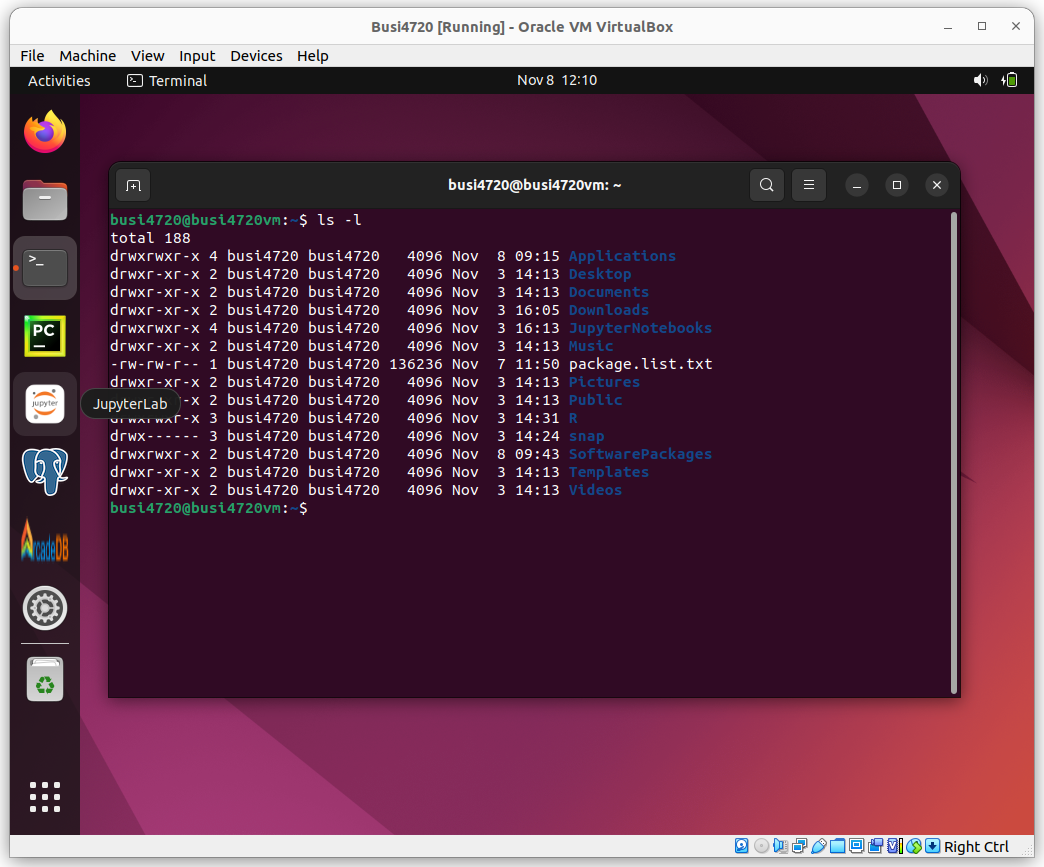
\includegraphics[height=3.1in]{screenshot1.png}
\end{frame}

\begin{frame}{Ubuntu Basics}
\begin{itemize}
  \item Version of Linux created and distributed by Canonical Inc. 
  \item Open source and multi-hardware support
  \item Long term support (LTS) versions released every 2 years, supported for 5 years
  \item Based on the Debian distribution
  \item User interface is called ''Gnome'' or ''Gnome Shell''
  \item Software is installed in packages
  \begin{itemize}
    \item Typically from the Ubuntu online repository or manually using Debian package files
    \item Use the ''apt'' command-line tool or the ''Synaptic'' graphical tool to manage packages
  \end{itemize}
\end{itemize}
\end{frame}

\begin{frame}{Ubuntu Basics \small [cont'd]}
\begin{itemize}
  \item Multi-user capable
  \begin{itemize}
    \item User files are in the directory/folder \texttt{''/home/busi4720/''}
  \end{itemize}
  \item Users have limited permissions to files and folders (read, write, eXecute)
  \item Users have limited privileges
  \begin{itemize}
    \item But some users are \emph{administrator} users and/or have \textbf{''sudo''} privileges
  \end{itemize}
\end{itemize}
\end{frame}

\begin{frame}[fragile]{The Ubuntu Command Line}
\footnotesize
In Ubuntu, you can open the Terminal using the key combination \colorbox{lightgray}{Ctrl-Alt-T}, or by selecting the Terminal icon from the side bar or the application list. You can also open a terminal from the file browser. \\
\underline{P}rint the \underline{w}orking \underline{d}irectory:
\scriptsize
\begin{bashcode}
busi4720@busi4720vm:~$ pwd
/home/busi4720
\end{bashcode}
\footnotesize

\underline{M}a\underline{k}e a folder/\underline{dir}ectory:
\scriptsize
\begin{bashcode}
busi4720@busi4720vm:~$ mkdir someFolder
\end{bashcode}
\footnotesize

\underline{C}hange the working \underline{d}irectory:
\scriptsize
\begin{bashcode}
busi4720@busi4720vm:~$ cd someFolder
busi4720@busi4720vm:~/someFolder$ cd ..
busi4720@busi4720vm:~$ cd ~
\end{bashcode}
\end{frame}

\begin{frame}[fragile]{The Ubuntu Command Line}
\footnotesize
\begin{block}{Special directory characters}
\begin{tabular}{l|l}
\texttt{\~} & User home directory \\
\texttt{.} & Current directory \\
\texttt{..} & Upwards in the directory tree \\
\texttt{/} & Root of directory tree \\
\end{tabular}
\end{block}
\begin{block}{Tips}
\begin{itemize}
  \item Autocompletion of file names with the ''\colorbox{lightgray}{tab}'' key (up to ambiguity)
  \item Recall earlier commands with the ''\colorbox{lightgray}{up arrow}'' key
  \item Search earlier commands with the ''\colorbox{lightgray}{Ctrl-R}'' key
  \item Cut/copy/paste with \colorbox{lightgray}{Ctrl-Shift-X}, \colorbox{lightgray}{Ctrl-Shift-C}, \colorbox{lightgray}{Ctrl-Shift-V}
\end{itemize}
\end{block}

\end{frame}


\begin{frame}[fragile]{The Ubuntu Command Line}
\footnotesize
\underline{L}i\underline{s}t folder/directory contents:
\tiny
\begin{bashcode}
busi4720@busi4720vm:~$ ls -l ~/Applications
total 4
drwxr-xr-x 8 busi4720 busi4720 4096 Nov  7 11:45 pycharm-community-2023.2.3
\end{bashcode}
\footnotesize
The results show the total size in kB, and a list of entries:
\begin{itemize}
  \item Type of entry (''d'' = directory)
  \item Permissions for owner (''rwx''), users in the same group (''r-x'') and other users (''r-x'')
  \item Names of owner and groups (''busi4720'')
  \item Size (in bytes)
  \item Last modification date and time
  \item File or directory name
\end{itemize}
\end{frame}

\begin{frame}[fragile]{The Ubuntu Command Line}
\footnotesize
Print a string of text:
\scriptsize
\begin{bashcode}
$ echo "To be or not to be"
To be or not to be
\end{bashcode}
\footnotesize

Redirect output to a file using the \emph{redirect} symbol ''\texttt{>}'':
\scriptsize
\begin{bashcode}
$ echo "To be or not to be" > someFile.txt
$ ls -l someFile.txt
-rw-rw-r-- 1 busi4720 busi4720 19 Nov  8 14:50 someFile.txt
\end{bashcode}
\footnotesize

Print contents of a file (''con\underline{cat}enate''):
\scriptsize
\begin{bashcode}
$ cat someFile.txt
To be or not to be
\end{bashcode}

\end{frame}


\begin{frame}[fragile]{The Ubuntu Command Line}
\footnotesize
\underline{C}o\underline{p}y a file:
\scriptsize
\begin{bashcode}
$ cp someFile.txt someCopy.txt
\end{bashcode}
\footnotesize

\underline{M}o\underline{v}e a file:
\scriptsize
\begin{bashcode}
$ mv someCopy.txt ~/someFolder
\end{bashcode}

Renaming is moving:
\begin{bashcode}
$ mv someFile.txt newName.txt
\end{bashcode}

\underline{R}e\underline{m}ove (delete) a file:
\begin{bashcode}
$ rm someFolder/someFile.txt
\end{bashcode}
\end{frame}

\begin{frame}[fragile]{The Ubuntu Command Line}
\footnotesize
Remove a directory recursively (i.e. remove all its contents first):\scriptsize
\begin{bashcode}
$ rm -r ~/someFolder
\end{bashcode}
\footnotesize
\alert{\emph{Use this very carefully!}} \\

%\vspace{5mm}

View the command line \underline{history}:
\scriptsize
\begin{bashcode}
$ history
    1  echo "To be or not to be"
    2  echo "To be or not to be" > someFile.txt
    3  ls -l someFile.txt
    4  less someFile.txt 
    5  cat someFile.txt
...
\end{bashcode}

\end{frame}

\begin{frame}[fragile]{The Ubuntu Command Line}
\footnotesize
Remove write permissions:
\begin{bashcode}
$ chmod -w newName.txt
\end{bashcode}

Add write permissions:
\begin{bashcode}
$ chmod +w newName.txt
\end{bashcode}

Add execute permissions:
\begin{bashcode}
$ chmode +x newName.txt
\end{bashcode}

\end{frame}

\begin{frame}[fragile]{The Ubuntu Command Line}
\footnotesize
Get the \underline{man}ual for a command:
\begin{bashcode}
$ man ls
\end{bashcode}

Find the processes running:
\begin{bashcode}
$ ps
\end{bashcode}

Find something in a file or input stream:
\begin{bashcode}
$ cat newName.txt | grep be
$ ls -l | grep .txt
$ history | grep .txt
\end{bashcode}

\emph{Note:} The vertical bar is called a \emph{''pipe''}, it pipes the output of one command as input into the next one
\end{frame}

\begin{frame}{Command Line Tutorials}
\begin{itemize}
\item \url{https://ubuntu.com/tutorials/command-line-for-beginners}
\item \url{https://www.digitalocean.com/community/tutorials/a-linux-command-line-primer}
\item \url{https://www.digitalocean.com/community/tutorial-series/getting-started-with-linux}
\end{itemize}
\end{frame}

\begin{frame}[allowframebreaks]{Hands-On Exercise}

The following are a set of connected exercises to help you practice your command line skills. Do them in the order listed.

\begin{enumerate}
\item Navigation and Listing
\begin{enumerate}
	\item Open the terminal and use the \texttt{pwd} command to print the current working directory.
	\item Use \texttt{ls} to list the contents of the current directory.
	\item Create a new directory named "Exercise1" using \texttt{mkdir}.
	\item Navigate into the "Exercise1" directory using \texttt{cd}.
\end{enumerate}
\item File Manipulation
\begin{enumerate}
	\item Create a new file named "file1.txt" inside the "Exercise1" directory using \texttt{touch}.
	\item Use \texttt{cat} to display the contents of "file1.txt".
	\item Append the text "Hello, Bash!" to "file1.txt" using \texttt{echo} and \texttt{>>}.
	\item Display the updated contents of "file1.txt" using \texttt{cat}.
\end{enumerate}
\item Removing and Renaming
\begin{enumerate}
	\item Remove "file1.txt" using the \texttt{rm} command.
	\item Create a copy of the "Exercise1" directory named "Exercise1\_backup" using \texttt{cp -r}.
	\item Remove the original "Exercise1" directory using \texttt{rm -r}.
\end{enumerate}
\item Directory Manipulation
\begin{enumerate}
	\item Recreate the "Exercise1" directory.
	\item Create three subdirectories inside "Exercise1" named "Subdir1", "Subdir2", and "Subdir3" using \texttt{mkdir}.
	\item List the contents of "Exercise1" to verify the creation of subdirectories.
\end{enumerate}
\item Searching and Filtering
\begin{enumerate}
	\item Create a file named "keywords.txt" inside "Exercise1" and add some random text.
	\item Use \texttt{grep} to search for a specific word (e.g., "Bash") in "keywords.txt".
	\item Create a new file named "filtered.txt" and use \texttt{grep} to filter lines containing the word you searched for in "keywords.txt".
\end{enumerate}
\item Process Management
\begin{enumerate}
	\item Use \texttt{ps} to display information about the current processes running on your system.
	\item Use \texttt{ps aux | grep bash} to filter and display information about Bash processes.
\end{enumerate}
\item Cleanup
\begin{enumerate}
	\item Remove the entire "Exercise1" directory and its contents using \texttt{rm -r}.
	\item Confirm that the "Exercise1" directory no longer exists by listing the contents of the current directory.
\end{enumerate}
\end{enumerate}
\end{frame}

\end{document}
